\chapter{基于改进的K-Shape时间序列聚类算法的气井分类算法}
在气井开采初期,气井一经投入使用就会打破气藏的静态平衡,诸如产量、压力和产物性质等关键参数便会随之变动。随着开采活动的进行,气水关系会愈加错综复杂。产水量将持续攀升,
低压井和产水井的数量不断增长,不同气井之间的差异会日益增大。这些因素会进一步增加气井的生产管理难度。为提高管理效能,企业需利用历史产量数据对气井进行有效分类。将
表现出相似生产特性的气井进行归类和分析,以帮助揭示它们的共同生产模式。使得企业能够迅速评估气井的生产状况,掌握关键生产特征,进而及时规划出针对性强的管理策略和治
理行动,以确保气井的顺畅运作。本章根据基于改进的分数阶时间序列聚类算法,根据气井的历史产量数据,对气井进行分类。首先对企业提供的报表数据进行整理和清洗,去除掉
报表中的冗余数据并将需要的信息批量提取出来。在获取了产量相关的序列后,使用改进的K-Shape时间序列聚类算法来对气井进行分类。
\section{问题分析}
企业气田的地质条件十分复杂,是典型的“低渗透、低压力、低丰度”气田。其单井产量小、压降速率快,随着气田不断进行规模开发,单井井数逐年增加,集气站也在不断的增大。
随着开采活动的不断进行,间歇井(气井按照固定的开关制度进行生产的气井)数量的也在逐步递增。气井在开采过程中,产量会随着井底污染、地层压力、地层渗透率、地层有效厚度
等的变化。不同气井产量随时间的变化差异巨大。因此,通过对气井产量进行时间序列聚类,可以将历史产量特性相似的井分为一类进行管理。帮助企业在后续开采、产气量预测
以及对间歇井的开关井策略制定时,根据类别分别制定方案。基于此需求,本章采用改进的K-Shape时间序列聚类算法,通过SBD来度量两变量之间的相似性,再根据数据的特征指定
初始簇心,通过迭代的方式不断更新,最终得到气井分类的结果。
\section{问题描述}
在气井产量的时间序列聚类分析中,我们的目标是将历史产量数据分组,以揭示不同气井的生产行为和潜在模式。具体而言,每个气井的时间序列数据可以表示为 \( X_i = \{x_{i1}, x_{i2}, \ldots, x_{im}\} \),其中 \( m \) 代表了时间序列的长度,即观测周期的总数。我们有 \( N \) 个这样的时间序列,形成了一个时间序列集合 \( X = \{x_1, x_2, \ldots, x_N\} \),我们的目标是将这些序列聚类到 \( k \) 个不同的类别中。
在聚类分析中,每个类别可能代表着不同的气井种类,正处在高产期和衰退期的井之间的时间序列差异巨大。假设k=3(但实际应用中需要根据肘部法则来确定最优的k值)则种类可以预先定义为类别 \( Y = \{0,1,2\} \)。因此,我们的任务是定义一个映射函数 \( f: X \to Y \),它可以将每个时间序列分配到这些预定义的类别中。
\section{基于改进的K-Shape时间序列聚类算法的气井分类算法}
\subsection{算法流程}
在传统的K-Shape聚类算法中,初始参考中心的选择是通过从样本集中随机挑选k个样本来进行的。这种随机选择方法可能会导致算法收敛于次优解,且每次运行结果都不一致,导致聚类结果不稳定。尤其是当数据集包含噪声或者离群点时。随机选取的初始中心可能不代表数据的真实结构,导致最终的聚类结果缺乏可解释性和准确性。此外,当样本集规模庞大时,随机选择方法可能导致算法收敛速度缓慢,影响聚类效率。
为了确定合适的聚类,通常采用多次实验的方法。本文结合领域知识和数据特点给出了一种改进策略:即根据数据特征选取初始中心点。具体如下:根据气井的历年累计产量,平均产量,
峰值产量的统计结果,对气井进行排序,并将其划分为k个区间,在每个区间内抽取中间的气井作为初始中心点。这样的方式可以使得初始的中心点更符合数据分布,从而实现
提高算法运行的稳定性。算法的流程图如图\ref{fig:K-Shape}所示。
\begin{figure}
    \centering
    % Requires \usepackage{graphicx}
    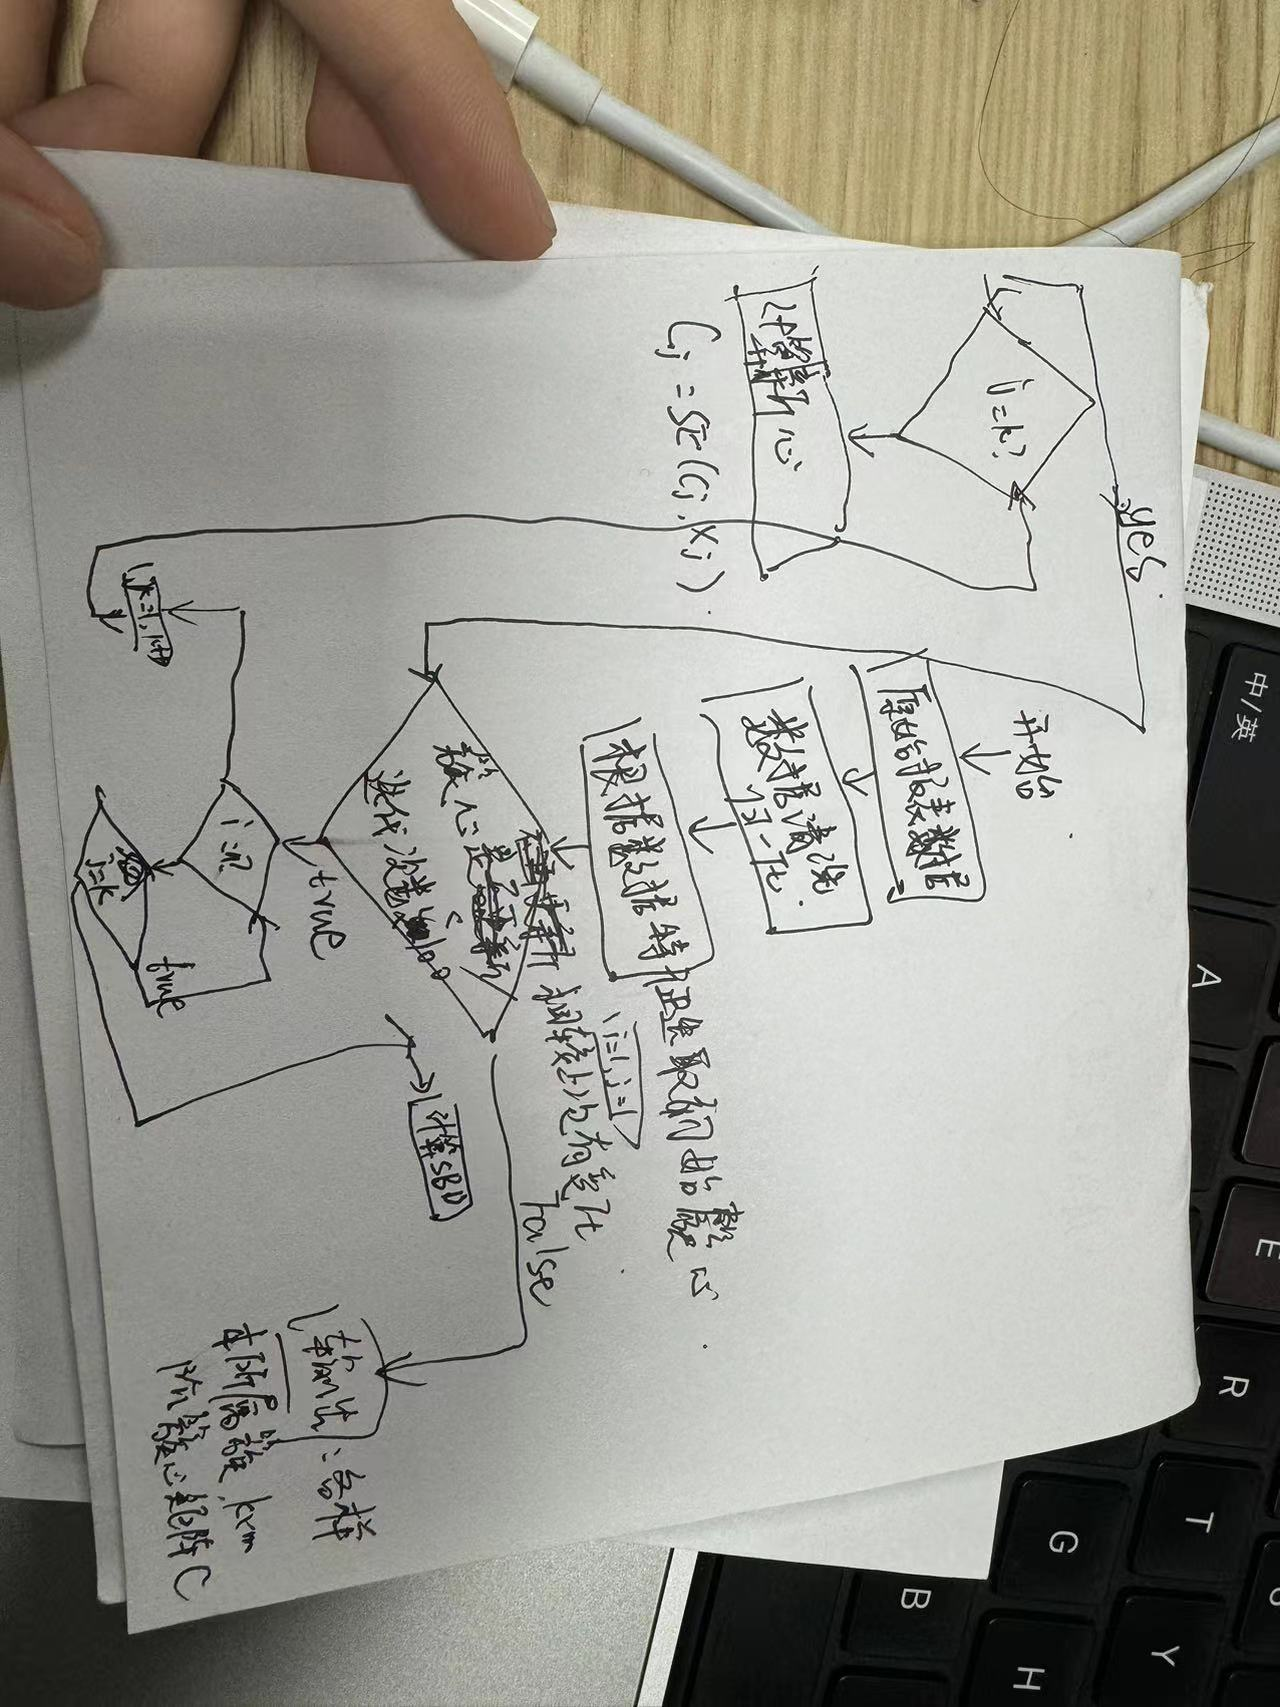
\includegraphics[scale=0.3,angle=0]{figure/K-Shape.jpg}\\
    \caption{基于改进的K-Shape时间序列聚类算法的气井分类算法流程图}
    \label{fig:K-Shape}
\end{figure}
初始报表的数据复杂且混乱,需要我们对其进行数据清理和整理,以形成一张规范的报表。在此基础上可以获取完整的产量数据,我们再根据第2章的方法对其进行归一化处理。然后
通过上文的方式选取初始参考中心。接下来,我们将通过不断的迭代更新簇心的方式来寻找最终的气井分类结果。这个过程将一直持续,直到簇心不再发生变化或者达到了预设
的最大迭代次数。最终,我们将得到一个高质量的气井分类结果。
\subsection{数据处理与分析}
原始数据集为单井日报文件,所给原始数据集时间跨度为:2012年8月3日至2022年8月15日,储存格式为一月的数据储存在一张excel多表中,一年共12张多表,每个
多表包含一月的数据,其中每日数据记录在一张excel表中,表中包含信息有所属井丛,井号,配产,生产时间(日累,月累,其中月累从2014年4月引入),油压,
套压(从2016年9月起开始引入),井口温度,注醇量(以井丛为单位),产气量(日产,月累,年累,历年年累),投产日期,备注(开关井信息)等。为进行批量读取处
理,需要先按照数据格式对所有报表进行划分,划分需考虑的因素包括不同的表头,报表的不同组织形式,不同的日期记录格式,剔除不需要的表(如一些影响批量读取的
总结性信息。如2012年的数据格式记录较为混乱,8,9两月的单井日报单井记录为了一个excel文件,10月,11月,12月三个月份的数据,由3个excel包含了各自月份的数据。
